\documentclass{standalone}
\usepackage[T1]{fontenc}
\usepackage[utf8]{inputenc}
\usepackage[auto]{microtype}
%\usepackage{cmbright}
\usepackage{arev}
\usepackage{amsmath, amssymb, amsfonts, icomma}
\usepackage[version=4]{mhchem}
\usepackage{tikz}
\usepackage{chemplants-tub}
\usepackage{xcolor}
%define stream tip, default is stealth
\setchpstreamtip{latex}
\setchpmainstreamthickness{thick}
%\setchpunitthickness{very thick}

\usetikzlibrary{shapes.geometric}

\pgfdeclarelayer{bg}    % declare background layer
\pgfsetlayers{bg,main}  % set the order of the layers (main is the standard layer)

% TABLEAU-10
\definecolor{Tab10-A}{RGB}{78, 121, 167}
\definecolor{Tab10-B}{RGB}{242, 142, 43}
\definecolor{Tab10-C}{RGB}{225, 87, 89}
\definecolor{Tab10-D}{RGB}{118, 183, 178}
\definecolor{Tab10-E}{RGB}{89, 161, 79}
\definecolor{Tab10-F}{RGB}{237, 201, 72}
\definecolor{Tab10-G}{RGB}{176, 122, 161}
\definecolor{Tab10-H}{RGB}{255, 157, 167}
\definecolor{Tab10-I}{RGB}{156, 117, 95}
\definecolor{Tab10-J}{RGB}{186, 176, 172}

\definecolor{AC}{RGB}{74, 84, 106}

\begin{document}
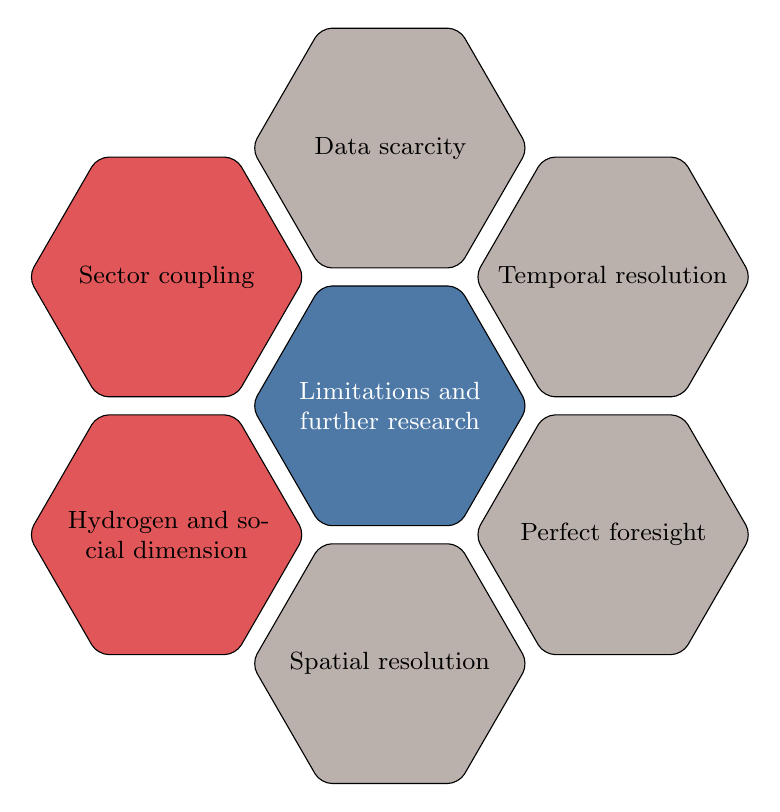
\begin{tikzpicture}[font=\small]

    \node[regular polygon, regular polygon sides=6,inner sep=2cm, rotate=30] (hexagon) {};

    \node[regular polygon,
	draw,
	regular polygon sides=6, rounded corners, fill=Tab10-A, minimum  width=100pt, text width= 100pt, inner sep=-20pt, align=center] (limits) at (hexagon.center) {\textcolor{white}{Limitations and further research}};

    \node[regular polygon,
	draw,
	regular polygon sides=6, rounded corners, fill=Tab10-J, minimum  width=100pt, text width= 100pt, inner sep=-20pt, outer sep=0pt, align=center] (data) at (hexagon.corner 1) {Data scarcity};

    \node[regular polygon,
	draw,
	regular polygon sides=6, rounded corners, fill=Tab10-C, minimum  width=100pt, text width= 100pt, inner sep=-20pt, outer sep=0pt, align=center] (data) at (hexagon.corner 2) {Sector coupling};

    \node[regular polygon,
	draw,
	regular polygon sides=6, rounded corners, fill=Tab10-C, minimum  width=100pt, text width= 100pt, inner sep=-20pt, outer sep=0pt, align=center] (data) at (hexagon.corner 3) {Hydrogen and social dimension};

    \node[regular polygon,
	draw,
	regular polygon sides=6, rounded corners, fill=Tab10-J, minimum  width=100pt, text width= 100pt, inner sep=-20pt, outer sep=0pt, align=center] (data) at (hexagon.corner 4) {Spatial resolution};

    \node[regular polygon,
	draw,
	regular polygon sides=6, rounded corners, fill=Tab10-J, minimum  width=100pt, text width= 100pt, inner sep=-20pt, outer sep=0pt, align=center] (data) at (hexagon.corner 5) {Perfect foresight};

    \node[regular polygon,
	draw,
	regular polygon sides=6, rounded corners, fill=Tab10-J, minimum  width=100pt, text width= 100pt, inner sep=-20pt, outer sep=0pt, align=center] (data) at (hexagon.corner 6) {Temporal resolution};

\end{tikzpicture}

\end{document}
